\Variant{05.10.2025 (1-smena)}
\QQ{1}{$x$ va $y$ ning ixtiyoriy natural qiymatlarida qaysi ifoda juft son böladi?
\Opts{$x^2+y^2$}{$xy+y$}{$(x+y)\cdot x$}{$(x+y)\cdot x\cdot y$}}
\QQ{2}{Hisoblang: $\{a\}$ — $a$ ning kasr qismi, $[a]$ — $a$ ning butun qismi.
\[\left\{\frac{\{-1{,}6\}}{[-1{,}6]}-\frac{[6{,}6]}{\{6{,}6\}}\right\}\]
\Opts{$-\dfrac15$}{$\dfrac45$}{$-10\dfrac15$}{$-\dfrac45$}}
\QQ{3}{Kinoteatrda har bir qatordagi örindiqlar soni qatorlardan $4$ ga köp. Jami örindiqlar soni $60$ ta. (Har bir qatordagi örindiqlar soni teng). Neçta qator bor?
\Opts{$10$}{$4$}{$6$}{$8$}}
\QQ{4}{Dökondagi köylakning dastlabki narxi $500\,000$ söm edi. Sotuvçi çegirma bilan $410\,000$ sömga sotdi. Sotuvçi neça foiz çegirma qilgan?
\Opts{$18\%$}{$36\%$}{$15\%$}{$24\%$}}
\QQ{5}{Soddalaştiring:
\[\frac{\sqrt{x^3}:\sqrt[5]x}{\sqrt[5]{x^4\cdot\sqrt{x^5}}}\]
\Opts{$1$}{$\dfrac1{x^2}$}{$\dfrac1x$}{$x$}}
\QQ{6}{Hisoblang:
\[\frac{\sqrt{3+2\sqrt2}-\sqrt{3-2\sqrt2}}{\sqrt{3+2\sqrt2}+\sqrt{3-2\sqrt2}}\]
\Opts{$2\sqrt2$}{$\sqrt2$}{$\dfrac{\sqrt2}2$}{$4$}}
\QQ{7}{Hisoblang:
\[\left(\sqrt{10-2\sqrt{21}}+\sqrt{10+2\sqrt{21}}\right)^2\]
\Opts{$25$}{$21$}{$27$}{$28$}}
\QQ{8}{Kamayuvçi arifmetik progressiyada $(a_5)^2+(a_6)^2=100$ va $S_9=54$ bölsa, $a_4$ ning qiymatini toping.
\Opts{$4$}{$18$}{$20$}{$10$}}
\QQ{9}{$a$, $b$, $c$ sonlari kamayuvçi geometrik progressiyaning ketma-ket hadlari. $a$; $1{,}5b$; $2c$ arifmetik progressiyaning ketma-ket uçta hadini taşkil etsa, geometrik progressiyaning maxrajini toping.
\Opts{$\dfrac23$}{$\dfrac34$}{$\dfrac13$}{$\dfrac12$}}
\QQ{10}{Agar $x=\sqrt[3]2$, $y=2$ va $a=3$ ga teng bölsa, $\dfrac{y^3\cdot x^{-a}-x^{-1}\cdot y\cdot x^{-2a+1}\cdot x^a}{x^{-a}\cdot y+x^{-a}}$ ifodaning qiymatini toping.
\Opts{$1$}{$4$}{$2$}{$3$}}
\QQ{11}{Ifodani soddalaştiring:
\[\left(\frac{\sqrt a-\sqrt b}{a+\sqrt{ab}}+\frac{\sqrt a+\sqrt b}{a-\sqrt{ab}}+\frac{2b}{b\sqrt a-a\sqrt a}\right)\cdot\left(\frac1{\sqrt a}-\frac1{\sqrt b}\right)\]
\Opts{$\dfrac2{\sqrt{ab}+b}$}{$\dfrac{-2}{\sqrt{ab}+a}$}{$\dfrac{-2}{\sqrt{ab}+b}$}{$\dfrac2{\sqrt{ab}+\sqrt b}$}}
\QQ{12}{$\dfrac{|\sin x|}{\sin x}=x$ tenglama neçta haqiqiy yeçimga ega?
\Opts{$1$}{$2$}{Haqiqiy yeçimga ega emas}{Çeksiz köp yeçimga ega}}
\QQ{13}{$\tg2\alpha+\ctg2\alpha+\tg6\alpha+\ctg6\alpha$ ni soddalaştiring.
\Opts{$\dfrac{4\cos^24\alpha}{\sin6\alpha}$}{$\dfrac{4\ctg4\alpha}{\sin12\alpha}$}{$\dfrac{8\cos^44\alpha}{\sin6\alpha}$}{$\dfrac{8\cos^24\alpha}{\sin12\alpha}$}}
\QQ{14}{Tengsizlik neçta butun yeçimga ega?
\[2^{\sqrt{4x}}-5\cdot2^{\sqrt x}<24\]
\Opts{$8$}{$9$}{$10$}{$11$}}
\QQ{15}{Tengsizlikning eng katta va eng kiçik butun yeçimlari yiğindisini toping.
\[x^{\log_6x^5}<216x^2\]
\Opts{$5$}{$6$}{$7$}{$8$}}
\QQ{16}{Tenglama neçta haqiqiy ildizga ega?
\[x^6+\sqrt{2021}\,x^3-1=0\]
\Opts{$4$}{$3$}{$2$}{haqiqiy ildizi mavjud emas}}
\QQ{17}{Tenglama neçta haqiqiy yeçimga ega?
\[(2x-4)^2\cdot(x+2)^2-\left(x^2-4\right)=3\]
\Opts{$1$}{$2$}{$3$}{$4$}}
\QQ{18}{Tengsizlikni yeçing:
\[\frac{x^3+1}{2x^2-3x+1}>1\]
\Opts{$\left(0;\,\dfrac12\right)\cup(1;\,\infty)$}{$\left(0;\,\dfrac14\right)\cup(1;\,\infty)$}{$\left(0;\,\dfrac12\right)\cup(2;\,\infty)$}{$(0;\,1)\cup(2;\,\infty)$}}
\QQ{19}{Tengsizlik neçta butun yeçimga ega?
\[\frac{x\cdot\sqrt{x+1}}{\sqrt{x+2}}\le0\]
\Opts{$2$}{$1$}{Haqiqiy yeçimga ega emas}{Çeksiz köp}}
\QQ{20}{$f(x)=ax^2+bx+c$ funksiyaning koeffitsiyentlari işoralarini aniqlang.
\qfig{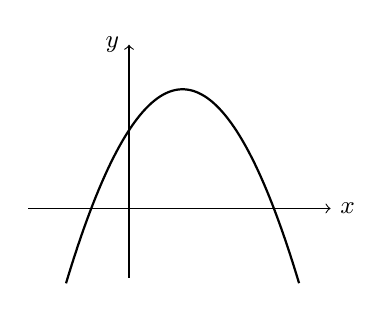
\begin{tikzpicture}[x=0.8cm,y=0.8cm,font=\small]
\draw[->] (-1.6,0)--(3.2,0) node[right] {$x$}; \draw[->] (0,-1.1)--(0,2.6) node[left] {$y$};
\draw[thick,domain=-1.0:2.7,samples=80] plot (\x,{-0.9*(\x+0.6)*(\x-2.3)});
\end{tikzpicture}}
\Opts{$a>0,\ b<0,\ c>0$}{$a<0,\ b<0,\ c>0$}{$a<0,\ b>0,\ c>0$}{$a<0,\ b>0,\ c<0$}}
\QQ{21}{Aniq integralni hisoblang:
\[\int_0^2x\cdot e^{x^2}\,dx\]
\Opts{$e^4-1$}{$2^{-1}\left(e^4-1\right)$}{$2^{-1}\left(e^2-1\right)$}{$1\dfrac12$}}
\QQ{22}{$y=x^2+4x-2$ funksiyaga $(x_0;\,y_0)$ nuqtada urinma ötkazilgan. Urinma $y=3x+4$ töğri çiziqqa parallel bölsa, $y_0$ ning qiymatini toping.
\Opts{$-3{,}75$}{$-2{,}25$}{$-2{,}5$}{$-2{,}75$}}
\QQ{23}{$f(x)=x(x+1)(x+2)(x+3)$ funksiyaning eng kiçik qiymatini toping.
\Opts{$0$}{$-\dfrac{15}{16}$}{$-1$}{$-1\dfrac18$}}
\QQ{24}{Markazi $O$ bölgan aylanaga $AB$ urinma va aylana markazidan ötuvçi $AE$ kesuvçi ötkazilgan ($D$ va $E$ — kesuvçining aylana bilan kesişiş nuqtalari, $D$ nuqta $A$ ga yaqin). Agar $AB=24$ va $AD=18$ bölsa, $AO$ ni toping.
\qfig{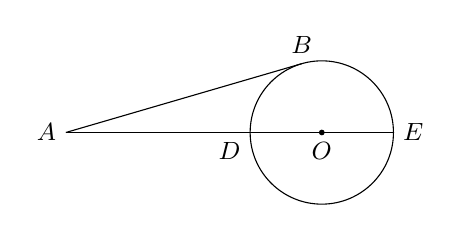
\begin{tikzpicture}[scale=0.13,font=\small]
\coordinate (O) at (0,0); \coordinate (A) at (-25,0); \coordinate (D) at (-7,0); \coordinate (E) at (7,0); \coordinate (B) at (-1.96,6.72);
\draw (O) circle (7); \draw (A)--(E); \draw (A)--(B); \fill (O) circle (8pt);
\node[left] at (A) {$A$}; \node[below left] at (D) {$D$}; \node[right] at (E) {$E$}; \node[above] at (B) {$B$}; \node[below] at (O) {$O$};
\end{tikzpicture}}
\Opts{$30$}{$32$}{$24$}{$25$}}
\QQ{25}{$ABC$ uçburçakda $AB$ tomondan $F$, $BC$ tomondan $E$ nuqta olingan bölib, $AE$ va $CF$ kesmalar $O$ nuqtada kesişadi. Agar $\dfrac{BF}{FA}=\dfrac13$, $\dfrac{BE}{BC}=\dfrac14$ va $AOC$ uçburçak yuzi $144$ cm$^2$ ga teng bölsa, $FOE$ uçburçak yuzini toping.
\qfig{\begin{tikzpicture}[scale=0.75,font=\small]
\coordinate (A) at (0,0); \coordinate (C) at (6,0); \coordinate (B) at (2.2,4.8); \coordinate (F) at (1.65,3.6); \coordinate (E) at (3.15,3.6); \coordinate (O) at (2.52,2.88);
\fill[qfill] (F)--(O)--(E)--cycle;
\draw (A)--(B)--(C)--cycle; \draw (A)--(E); \draw (C)--(F); \draw (F)--(E);
\node[below left] at (A) {$A$}; \node[above] at (B) {$B$}; \node[below right] at (C) {$C$}; \node[left] at (F) {$F$}; \node[right] at (E) {$E$}; \node[below] at (O) {$O$};
\node at (3,0.8) {$144$ cm$^2$};
\end{tikzpicture}}
\Opts{$16$}{$9$}{$12$}{$25$}}
\QQ{26}{Uçburçakning tomonlari $AB=5$, $BC=4$ va $AC=3$ ga teng. $C$ uçidan $AB$ tomonga $CD$ bissektrisa va $CM$ mediana tuşirilgan. $M$ va $D$ nuqtalar orasidagi masofani toping.
\Opts{$\dfrac57$}{$\dfrac5{14}$}{$\dfrac7{10}$}{$\dfrac9{35}$}}
\QQ{27}{$ABCD$ trapetsiyaning diagonallari $O$ nuqtada kesişadi. Agar $\dfrac{BO}{BD}=\dfrac13$ va $ABCD$ trapetsiya yuzi $162$ ga teng bölsa, $ABO$ uçburçak yuzini toping.
\qfig{\begin{tikzpicture}[scale=0.75,font=\small]
\coordinate (A) at (0,0); \coordinate (D) at (6,0); \coordinate (B) at (1,3); \coordinate (C) at (4,3); \coordinate (O) at (2.667,2);
\fill[qfill] (A)--(B)--(O)--cycle;
\draw (A)--(B)--(C)--(D)--cycle; \draw (A)--(C); \draw (B)--(D);
\node[below left] at (A) {$A$}; \node[above left] at (B) {$B$}; \node[above right] at (C) {$C$}; \node[below right] at (D) {$D$}; \node[below] at (O) {$O$};
\end{tikzpicture}}
\Opts{$18$}{$36$}{$42$}{$27$}}
\QQ{28}{$ABCDE$ muntazam beşburçakning barça diagonallari kesişişidan $FGHKL$ muntazam beşburçak hosil qilindi. Agar $FG=2$ ga teng bölsa, $ABCDE$ muntazam beşburçak perimetrini toping.
\qfig{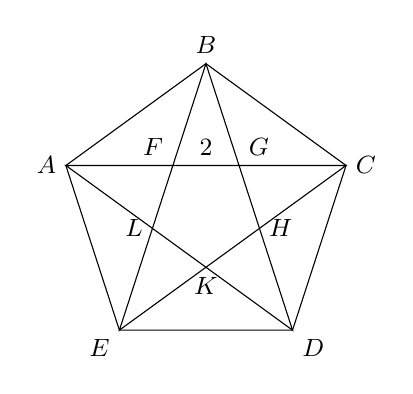
\begin{tikzpicture}[scale=0.42,font=\small]
\coordinate (B) at (0.000,4.454); \coordinate (C) at (4.236,1.376); \coordinate (D) at (2.618,-3.603); \coordinate (E) at (-2.618,-3.603); \coordinate (A) at (-4.236,1.376);
\coordinate (F) at (-1.000,1.376); \coordinate (G) at (1.000,1.376); \coordinate (H) at (1.618,-0.526); \coordinate (K) at (0.000,-1.701); \coordinate (L) at (-1.618,-0.526);
\draw (A)--(B)--(C)--(D)--(E)--cycle; \draw (A)--(C)--(E)--(B)--(D)--cycle;
\node[above] at (B) {$B$}; \node[right] at (C) {$C$}; \node[below right] at (D) {$D$}; \node[below left] at (E) {$E$}; \node[left] at (A) {$A$};
\node[above left] at (F) {$F$}; \node[above right] at (G) {$G$}; \node[right] at (H) {$H$}; \node[below] at (K) {$K$}; \node[left] at (L) {$L$}; \node[above] at (0,1.376) {$2$};
\end{tikzpicture}}
\Opts{$20$}{$5\left(3-\sqrt5\right)$}{$5\left(3+\sqrt5\right)$}{$25$}}
\QQ{29}{$A(-5;\,-3)$, $B(-2;\,5)$, $C(7;\,6)$ va $D(m;\,n)$ nuqtalar parallelogrammning uçlari bölsa, $\overrightarrow{AC}$ va $\overrightarrow{DB}$ vektorlar orasidagi burçak kosinusini toping.
\Opts{$-\dfrac3{5\sqrt{85}}$}{$\dfrac3{5\sqrt{85}}$}{$-\dfrac{\sqrt{45}}{10}$}{$\dfrac{\sqrt{45}}{10}$}}
\QQ{30}{$ABC$ töğri burçakli uçburçak tekisligiga $C$ uçiga $CD$ perpendikulyar ötkazilgan. Katetlari $AC=15$, $BC=20$ va $CD=35$ ga teng bölsa, $D$ nuqtadan $AB$ tomongaça bölgan eng qisqa masofani toping.
\Opts{$36$}{$37$}{$40$}{$39$}}
\QQ{31}{Restoranda $8$ xil salatga mayonez qöşilgan, $5$ xil salatga piyoz qöşilgan, $2$ xil salatga ham mayonez, ham piyoz qöşilgan salat tayyorlanadi. Restoranda jami $14$ xil salat tayyorlansa, neça xil salatga mayonez va piyoz qöşilmagan böladi?
\Opts{$2$}{$3$}{$4$}{$5$}}
\QQ{32}{Neçta uç xonali natural sonlarda faqat bitta $7$ raqami qatnaşadi?
\Opts{$81$}{$225$}{$144$}{$72$}}
\QQ{33}{\Moslash{Şar içiga bir vaqtning özida eng katta hajmli konus va eng katta hajmli silindr içki çizilgan.}{A) $\dfrac{8\sqrt3}{27}$\par B) $\dfrac{\sqrt6}9$\par C) $\dfrac{4\sqrt3}3$\par D) $\dfrac{2\sqrt3}3$\par E) $\dfrac{\sqrt6}3$\par F) $\dfrac{4\sqrt3}{27}$}{Konus asosi radiusining silindr asosi radiusiga nisbatini $\left(\dfrac{R_k}{R_s}\right)$ toping.}{Konus hajmining silindr hajmiga nisbatini $\left(\dfrac{V_k}{V_s}\right)$ toping.}{Konus yon sirtining silindr yon sirtiga nisbatini $\left(\dfrac{S_{\text{yon}\,k}}{S_{\text{yon}\,s}}\right)$ toping.}}
\QQ{36}{Tenglamani yeçing:
\[x=9-\sqrt{9-\sqrt x}\]
\AB{Tenglama neçta haqiqiy ildizga ega?}{Tenglama haqiqiy ildizlari yiğindisini toping (Agar u bitta bölsa, şu ildizini toping).}}
\QQ{37}{Tenglamani yeçing:
\[\sin x+2\sin2x+\sin3x=|1+2\cos x+\cos2x|\]
\AB{Tenglama $[-2\pi;\,2\pi]$ oraliqda neçta yeçimga ega?}{Tenglamaning $[0;\,2\pi]$ oraliqdagi ildizlari yiğindisini toping.}}
\QQ{38}{$f(x)$ funksiya uçun quyidagi tenglik örinli:
\[4f(x)+\frac23\left(x^2+2\right)f\left(x-\frac2x\right)=x^3+1\]
\AB{$f(1)-f(-1)$ ning qiymatini toping.}{$f(2)-f(-2)$ ning qiymatini toping.}}
\QQ{39}{$f(x)=-x^3+2x^2+5x-6{,}5$ va $g(x)=0{,}5(x-1)^2+a$ funksiyalar umumiy bir neçta nuqtaga ega. Ulardan bitta nuqtasida urinadi.
\AB{$a$ ning eng katta qiymatini toping.}{$a$ ning eng katta qiymatidagi uriniş nuqtasining koordinatalari yiğindisini toping.}}
\QQ{40}{$f(x)=ax^2+bx+c$ va $g(x)=|x+m|+n$ funksiyalar grafiklari $Oy$ öqida va $(6;\,10)$ nuqtada kesişadi. Parabolaning simmetriya öqi $x=4$.
\qfig{\begin{tikzpicture}[x=0.5cm,y=0.3cm,font=\small]
\fill[qfill] plot[domain=0:6,samples=60] (\x,{-\x*\x/2+4*\x+4}) -- (0,4) -- cycle;
\draw[->] (-3.5,0)--(10,0) node[right] {$x$}; \draw[->] (0,-1.5)--(0,13.5) node[left] {$y$};
\draw[thick,domain=-0.95:8.95,samples=100] plot (\x,{-\x*\x/2+4*\x+4});
\draw[thick] (-3.3,4.3)--(-1.5,2.5)--(8,12);
\draw[dashed] (4,0)--(4,12); \node[below] at (4,0) {$4$};
\fill (0,4) circle (2.5pt); \fill (6,10) circle (2.5pt); \node[right] at (6.2,10) {$(6;\,10)$};
\node[right] at (8.4,6) {$f(x)=ax^2+bx+c$}; \node[left] at (-1.6,5.4) {$g(x)=|x+m|+n$};
\end{tikzpicture}}
\AB{$f(x)$ funksiyaning eng katta qiymatini toping.}{Böyalgan soha yuzini toping.}}
\QQ{41}{$ABC$ töğri burçakli uçburçakning $AH$ balandligi ikkita $ABH$ va $AHC$ töğri burçakli uçburçaklarga ajratadi. $ABH$ va $AHC$ uçburçaklarga içki çizilgan aylanalar markazlaridan ötuvçi töğri çiziq $AB$ va $AC$ tomonlarni mos ravişda $M$ va $N$ nuqtalarda kesib ötadi. Agar $BH=4$ cm va $HC=9$ cm ekanligi maʼlum bölsa,
\qfig{\begin{tikzpicture}[scale=0.42,font=\small]
\coordinate (B) at (-4,0); \coordinate (H) at (0,0); \coordinate (C) at (9,0); \coordinate (A) at (0,6); \coordinate (M) at (-3.328,1.008); \coordinate (N) at (4.992,2.672);
\coordinate (O1) at (-1.394,1.394); \coordinate (O2) at (2.092,2.092);
\fill[qfill] (A)--(M)--(N)--cycle;
\draw (A)--(B)--(C)--cycle; \draw (A)--(H); \draw (O1) circle (1.394); \draw (O2) circle (2.092); \draw (M)--(N);
\fill (O1) circle (3pt); \fill (O2) circle (3pt);
\draw (0,0.4)--(0.4,0.4)--(0.4,0);
\node[above] at (A) {$A$}; \node[below left] at (B) {$B$}; \node[below right] at (C) {$C$}; \node[below] at (H) {$H$}; \node[left] at (M) {$M$}; \node[above right] at (N) {$N$};
\node[below] at (O1) {$O_1$}; \node[below] at (O2) {$O_2$}; \node[below] at (-2,0) {$4$}; \node[below] at (4.5,0) {$9$};
\end{tikzpicture}}
\AB{$\angle ANM=\alpha$ bölsa, $\tg\alpha$ ni toping.}{$AMN$ uçburçak yuzini (cm$^2$) toping.}}
\QQ{42}{$ABCD$ kvadratga yuzalari $16$ va $9$ ga teng bölgan $AGFE$ va $MCLK$ kvadratlar içki çizildi. Bunda $G$ nuqta $AB$ tomonda, $E$ nuqta $AD$ tomonda, $L$ nuqta $CD$ tomonda, $M$ nuqta $BC$ tomonda yotadi. Agar $FK=\sqrt2$ ga teng bölsa,
\AB{$ABCD$ kvadrat yuzining eng katta qiymatini toping.}{$ABCD$ kvadrat eng kiçik yuzaga ega bölsa, $FD$ ni toping.}}
\QQ{43}{$ABCD$ kvadrat içida $E$ nuqta tanlab olingan. Agar $\angle EAC=\angle ECD=15^\circ$, $E$ nuqta kvadratning tomonida yotmaydi. $AC$ va $BE$ kesmalar $O$ nuqtada kesişadi.
\AB{$\angle ABE$ ni toping.}{Agar $OE=\sqrt3-1$ ga teng bölsa, $S_{OEC}$ uçburçak yuzini toping.}}
\QQ{44}{Konusga asosi kvadrat bölgan parallelepiped içki çizilgan. Konus balandligi asosining diametriga teng. Parallelepiped yon sirti $24-16\sqrt2$ ga teng va parallelepiped balandligi asosining tomonidan $2$ marta katta.
\qfig{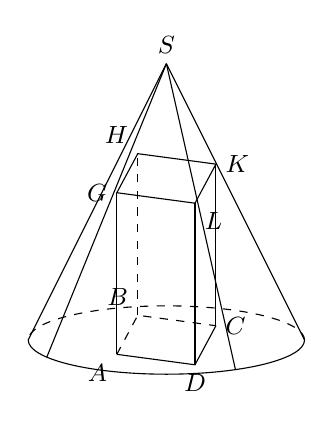
\begin{tikzpicture}[scale=0.62,font=\small]
\coordinate (S) at (0,5.66);
\coordinate (A) at (-1.015,-0.293); \coordinate (D) at (0.586,-0.507); \coordinate (C) at (1.015,0.293); \coordinate (B) at (-0.586,0.507);
\coordinate (G) at (-1.015,3.017); \coordinate (L) at (0.586,2.803); \coordinate (K) at (1.015,3.603); \coordinate (H) at (-0.586,3.817);
\draw (-2.83,0) arc (180:360:2.83 and 0.7); \draw[dashed] (2.83,0) arc (0:180:2.83 and 0.7);
\draw (S)--(-2.83,0); \draw (S)--(2.83,0);
\draw[thin] (S)--(-2.451,-0.354); \draw[thin] (S)--(1.415,-0.606);
\draw (A)--(D)--(C); \draw[dashed] (A)--(B)--(C); \draw[dashed] (B)--(H);
\draw (A)--(G); \draw (D)--(L); \draw (C)--(K); \draw (G)--(L)--(K)--(H)--cycle;
\node[above] at (S) {$S$}; \node[below left] at (A) {$A$}; \node[below] at (D) {$D$}; \node[right] at (C) {$C$}; \node[above left] at (B) {$B$};
\node[left] at (G) {$G$}; \node[below right] at (L) {$L$}; \node[right] at (K) {$K$}; \node[above left] at (H) {$H$};
\end{tikzpicture}}
\AB{Konus yon sirtini toping.}{$\angle GSK$ burçak sinusini toping.}}
\QQ{45}{Aylana va uçi şu aylana markazida bölgan parabola $C$ va $D$ nuqtalarda kesişadi. $O$ — aylana markazi. Aylana radiusi $3$ cm va $D$ nuqtadan $AB$ diametrga ötkazilgan perpendikulyar uzunligi $2$ cm ga teng.
\qfig{\begin{tikzpicture}[scale=0.62,font=\small]
\fill[qfill] plot[domain=0:2.236,samples=40] (\x,{0.4*\x*\x}) -- (2.236,0) -- cycle;
\draw (0,0) circle (3); \draw (-3,0)--(3,0);
\draw[thick,domain=-3.6:3.6,samples=80] plot (\x,{0.4*\x*\x});
\draw (2.236,0)--(2.236,2); \draw (2.236,0.25)--(2.486,0.25)--(2.486,0);
\fill (0,0) circle (1.5pt);
\node[left] at (-3,0) {$A$}; \node[right] at (3,0) {$B$}; \node[below] at (0,0) {$O$}; \node[above right] at (2.236,2) {$D$}; \node[above left] at (-2.236,2) {$C$};
\node[right] at (2.236,1) {$2$}; \node[below] at (-1.5,0) {$3$};
\end{tikzpicture}}
\AB{$CD$ kesma uzunligini (cm) toping.}{Böyalgan soha yuzini (cm$^2$) toping.}}
\Javoblar{D B C A A C D C D C C B D B B C D A A C B A C D B B B C A B B B D A E}{%
\OK{36}{$1$}{$\dfrac{19-\sqrt{37}}2$}\OK{37}{$10$}{$\dfrac{13\pi}3$}\OK{38}{$1$}{$3$}\OK{39}{$3$}{$5{,}5$}\OK{40}{$12$}{$18$}%
\OK{41}{$1$}{$18$}\OK{42}{$64$}{$2\sqrt5$}\OK{43}{$60^\circ$}{$\dfrac12$}\OK{44}{$\dfrac{\sqrt5\,\pi}2$}{$\dfrac45$}\OK{45}{$2\sqrt5$}{$\dfrac{2\sqrt5}3$}}
